\section{Casos de uso}

\begin{figure}[H]
  \centering
  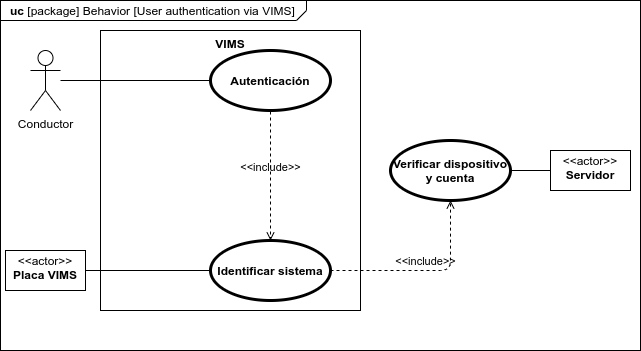
\includegraphics[width=\linewidth]{diagrams/UseCases-UC1 - auth.png}
  \caption{Caso de uso \texttt{01} -- \textit{autenticación}.}
  \label{uc:auth}
\end{figure}

\begin{table}[H]
  \centering
  \begin{tabularx}{\textwidth}{|c|c|X|}
    \hline
    \texttt{01}                                & \multicolumn{2}{c|}{\textit{Autenticación}}                                                                                                                                                                                                                 \\
    \hline
    \textbf{Descripción}                       & \multicolumn{2}{X|}{La placa identificará de forma inequívoca al conductor (usuario) y a sí misma frente al servidor.}                                                                                                                                      \\
    \hline
    \multirow{5}{*}{\textbf{Secuencia normal}} & \textbf{Paso}                                                                                                          & \textbf{Acción}                                                                                                                    \\
    \cline{2-3}
                                               & 1                                                                                                                      & \multicolumn{1}{L|}{El usuario se autentica contra la placa con su cuenta personal ya creada.}                                     \\
    \cline{2-3}
                                               & 2                                                                                                                      & \multicolumn{1}{L|}{La placa \ac{VIMS} recoge la información del usuario y la envía al servidor junto con su identificador único.} \\
    \cline{2-3}
                                               & 3                                                                                                                      & \multicolumn{1}{L|}{El servidor verifica que la cuenta del usuario existe y se asocia la información al dispositivo.}              \\
    \cline{2-3}
                                               & 4                                                                                                                      & \multicolumn{1}{L|}{La placa almacena la información del usuario y finaliza el proceso de inicio de sesión.}                       \\
    \hline
    \multirow{2}{*}{\textbf{Excepciones}}      & \textbf{Paso}                                                                                                          & \textbf{Acción}                                                                                                                    \\
    \cline{2-3}
                                               & 2                                                                                                                      & \multicolumn{1}{L|}{La placa no cuenta con conexión a la red o el servidor no está disponible.}                                    \\
    \cline{2-3}
                                               & 3                                                                                                                      & \multicolumn{1}{L|}{La cuenta del usuario no existe.}                                                                              \\
    \hline
  \end{tabularx}
\end{table}

\noindent\rule{\linewidth}{.2pt}

\begin{figure}[H]
  \centering
  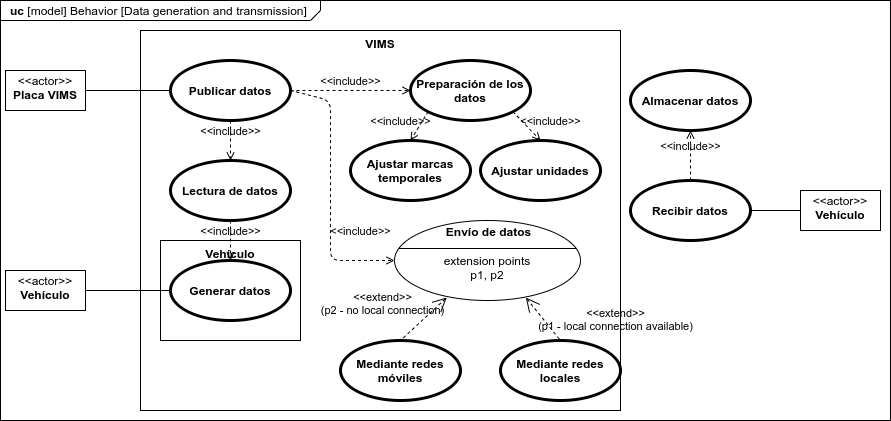
\includegraphics[width=\linewidth]{diagrams/UseCases-UC2 - data.png}
  \caption{Casos de uso \texttt{02} -- \textit{generación y transmisión de datos}.}
  \label{uc:data}
\end{figure}

\begin{table}[H]
  \centering
  \begin{tabularx}{\textwidth}{|c|c|X|}
    \hline
    \texttt{02}                                & \multicolumn{2}{c|}{\textit{Generación y transmisión de datos}}                                                                                                                                                                                                                                                                                                   \\
    \hline
    \textbf{Descripción}                       & \multicolumn{2}{X|}{El dispositivo \ac{VIMS} recibirá los datos del vehículo al que está conectado y los preparará para una posterior transmisión al servidor remoto de almacenamiento y gestión.}                                                                                                                                                                \\
    \hline
    \multirow{5}{*}{\textbf{Secuencia normal}} & \textbf{Paso}                                                                                                                                                                                      & \textbf{Acción}                                                                                                                                              \\
    \cline{2-3}
                                               & 1                                                                                                                                                                                                  & \multicolumn{1}{L|}{La placa \ac{VIMS} recibe los datos que el vehículo está generando de forma continuada.}                                                 \\
    \cline{2-3}
                                               & 2                                                                                                                                                                                                  & \multicolumn{1}{L|}{Los datos recibidos se preparan para el envío, ajustando cierta información y añadiendo valores como la cuenta asociada a dichos datos.} \\
    \cline{2-3}
                                               & 3                                                                                                                                                                                                  & \multicolumn{1}{L|}{Mediante el uso de redes móviles o locales, según disponibilidad, se envían los datos al servidor.}                                      \\
    \cline{2-3}
                                               & 4                                                                                                                                                                                                  & \multicolumn{1}{L|}{El servidor recibe la información transmitida por el sistema y la almacena para una posterior visualización y tratamiento.}              \\
    \hline
    \multirow{6}{*}{\textbf{Excepciones}}      & \textbf{Paso}                                                                                                                                                                                      & \textbf{Acción}                                                                                                                                              \\
    \cline{2-3}
                                               & 1                                                                                                                                                                                                  & \multicolumn{1}{L|}{El vehículo no está conectado o no transmite datos.}                                                                                     \\
    \cline{2-3}
                                               & 2                                                                                                                                                                                                  & \multicolumn{1}{L|}{Todavía no hay ninguna cuenta asociada a la placa \ac{VIMS}.}                                                                            \\
    \cline{2-3}
                                               & 3.1                                                                                                                                                                                                & \multicolumn{1}{L|}{No hay redes móviles disponibles, se intenta transmitir por redes locales.}                                                              \\
    \cline{2-3}
                                               & 3.2                                                                                                                                                                                                & \multicolumn{1}{L|}{No hay redes locales disponibles, se intenta transmitir por redes móviles.}                                                              \\
    \cline{2-3}
                                               & 3.3                                                                                                                                                                                                & \multicolumn{1}{L|}{No hay redes disponibles, se almacenan los datos para su posterior transmisión.}                                                         \\
    \hline
  \end{tabularx}
\end{table}

\noindent\rule{\linewidth}{.2pt}

\begin{figure}[H]
  \centering
  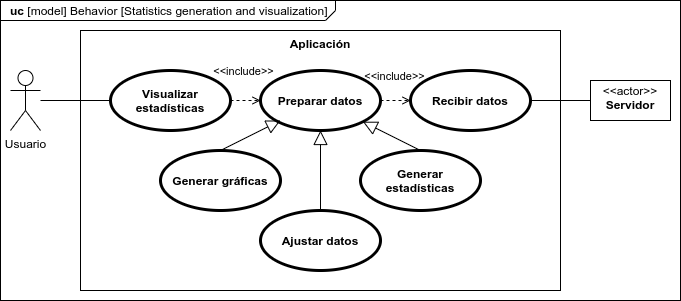
\includegraphics[width=\linewidth]{diagrams/UseCases-UC3 - stats.png}
  \caption{Caso de uso \texttt{03} -- \textit{generación de estadísticas}.}
  \label{uc:stats}
\end{figure}

\begin{table}[H]
  \centering
  \begin{tabularx}{\textwidth}{|c|c|X|}
    \hline
    \texttt{03}                                & \multicolumn{2}{c|}{\textit{Generación de estadísticas}}                                                                                                                                                                                                                                                                \\
    \hline
    \textbf{Descripción}                       & \multicolumn{2}{X|}{El servidor, en conjunción con el resto de elementos del sistema, preparará los datos para generar información estadística útil para el usuario.}                                                                                                                                                   \\
    \hline
    \multirow{4}{*}{\textbf{Secuencia normal}} & \textbf{Paso}                                                                                                                                                         & \textbf{Acción}                                                                                                                                 \\
    \cline{2-3}
                                               & 1                                                                                                                                                                     & \multicolumn{1}{L|}{El usuario solicita al servidor visualizar estadísticas con respecto a sus vehículos.}                                      \\
    \cline{2-3}
                                               & 2                                                                                                                                                                     & \multicolumn{1}{L|}{El servidor prepara los datos y genera distintos tipos de información estadística visual basados en tablas, gráficos, etc.} \\
    \cline{2-3}
                                               & 3                                                                                                                                                                     & \multicolumn{1}{L|}{El usuario recibe la información estadística ajustada a su cuenta.}                                                         \\
    \hline
    \multirow{4}{*}{\textbf{Excepciones}}      & \textbf{Paso}                                                                                                                                                         & \textbf{Acción}                                                                                                                                 \\
    \cline{2-3}
                                               & 1.1                                                                                                                                                                   & \multicolumn{1}{L|}{El usuario no está autenticado.}                                                                                            \\
    \cline{2-3}
                                               & 1.2                                                                                                                                                                   & \multicolumn{1}{L|}{El usuario no cuenta con ningún dispositivo \ac{VIMS} asociado.}                                                            \\
    \cline{2-3}
                                               & 2                                                                                                                                                                     & \multicolumn{1}{L|}{Todavía no se ha registrado ningún dato.}                                                                                   \\
    \hline
  \end{tabularx}
\end{table}

\noindent\rule{\linewidth}{.2pt}

\begin{figure}[H]
  \centering
  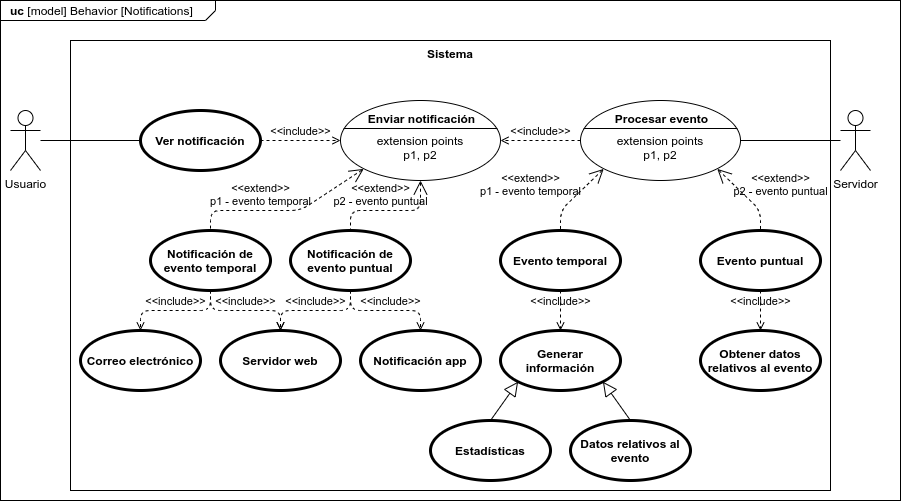
\includegraphics[width=\linewidth]{diagrams/UseCases-UC4 - notifications.png}
  \caption{Caso de uso \texttt{04} -- \textit{envío de notificaciones}.}
  \label{uc:notifications}
\end{figure}

\begin{table}[H]
  \centering
  \begin{tabularx}{\textwidth}{|c|c|X|}
    \hline
    \texttt{04}                                 & \multicolumn{2}{c|}{\textit{Envío de notificaciones}}                                                                                                                                                                                                                                                                                                                                                                                   \\
    \hline
    \textbf{Descripción}                        & \multicolumn{2}{X|}{El servidor, en conjunción con el resto de elementos del sistema, detecta ciertos eventos y actúa generando una notificación que envía al usuario.}                                                                                                                                                                                                                                                                 \\
    \hline
    \multirow{17}{*}{\textbf{Secuencia normal}} & \textbf{Paso}                                                                                                                                                           & \textbf{Acción}                                                                                                                                                                                                                                               \\
    \cline{2-3}
                                                & 1                                                                                                                                                                       & \multicolumn{1}{L|}{El servidor en un instante puntual produce y procesa un evento.}                                                                                                                                                                          \\
    \cline{2-3}
                                                & 1.1                                                                                                                                                                     & \multicolumn{1}{L|}{Si el evento se ha producido por un hecho (p.e.: repostar, finalizar un viaje, \dots), es un evento puntual sobre el cual se envía información relativa al mismo y al contexto (estadísticas del depósito, información del viaje, etc.).} \\
    \cline{2-3}
                                                & 1.2                                                                                                                                                                     & \multicolumn{1}{L|}{Si el evento se ha producido porque ha pasado un lapso de tiempo, es un evento temporal. El servidor generará estadísticas relativas a ese lapso de tiempo y mandará esa notificación.}                                                   \\
    \cline{2-3}
                                                & 2                                                                                                                                                                       & \multicolumn{1}{L|}{Se envía una notificación al usuario con los datos relativos al evento.}                                                                                                                                                                  \\
    \cline{2-3}
                                                & 2.1                                                                                                                                                                     & \multicolumn{1}{L|}{Si es un evento puntual, la notificación se envía a todos los medios: correo electrónico, servidor web y aplicación.}                                                                                                                     \\
    \cline{2-3}
                                                & 2.2                                                                                                                                                                     & \multicolumn{1}{L|}{Si es un evento temporal, la notificación se envía solo al correo electrónico y al servidor web.}                                                                                                                                         \\
    \cline{2-3}
                                                & 3                                                                                                                                                                       & \multicolumn{1}{L|}{El usuario recibe la notificación en alguno de los tres medios.}                                                                                                                                                                          \\
    \hline
  \end{tabularx}
\end{table}

\noindent\rule{\linewidth}{.2pt}

\begin{figure}[H]
  \centering
  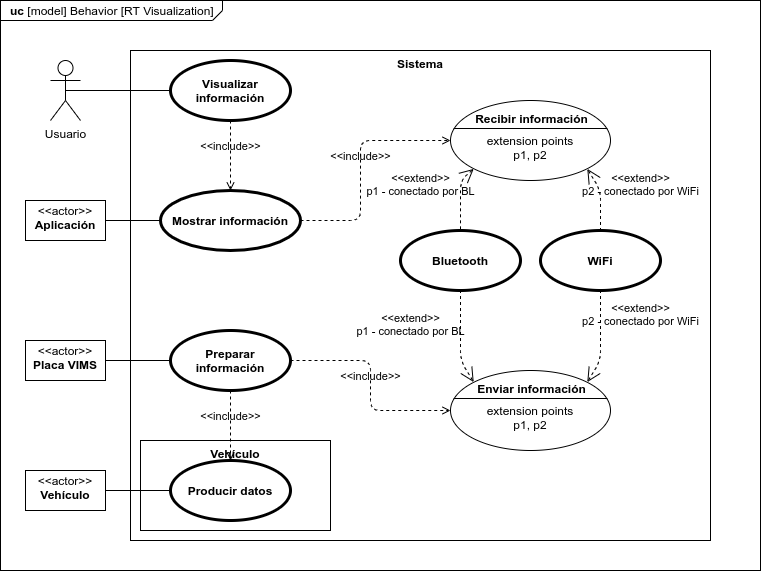
\includegraphics[width=\linewidth]{diagrams/UseCases-UC5 - visualization.png}
  \caption{Caso de uso \texttt{05} -- \textit{visualización en tiempo real}}
  \label{uc:visualization}
\end{figure}

\begin{table}[H]
  \centering
  \begin{tabularx}{\textwidth}{|c|c|X|}
    \hline
    \texttt{05}                                & \multicolumn{2}{c|}{\textit{Visualización en tiempo real}}                                                                                                                                                                                         \\
    \hline
    \textbf{Descripción}                       & \multicolumn{2}{X|}{Un usuario podrá visualizar información en tiempo real sobre su vehículo mediante la aplicación.}                                                                                                                              \\
    \hline
    \multirow{8}{*}{\textbf{Secuencia normal}} & \textbf{Paso}                                                                                                         & \textbf{Acción}                                                                                                            \\
    \cline{2-3}
                                               & 1                                                                                                                     & \multicolumn{1}{L|}{El usuario solicita visualizar información sobre el vehículo desde la aplicación.}                     \\
    \cline{2-3}
                                               & 2                                                                                                                     & \multicolumn{1}{L|}{La aplicación recibe la información de la placa \ac{VIMS} usando redes \ac{PAN}.}                      \\
    \cline{2-3}
                                               & 3                                                                                                                     & \multicolumn{1}{L|}{La placa \ac{VIMS} prepara la información que recibe del vehículo y la transmite hacia la aplicación.} \\
    \hline
    \multirow{12}{*}{\textbf{Excepciones}}     & \textbf{Paso}                                                                                                         & \textbf{Acción}                                                                                                            \\
    \cline{2-3}
                                               & 1.1                                                                                                                   & \multicolumn{1}{L|}{El usuario no está autenticado.}                                                                       \\
    \cline{2-3}
                                               & 1.2                                                                                                                   & \multicolumn{1}{L|}{El usuario no cuenta con ningún dispositivo \ac{VIMS} asociado.}                                       \\
    \cline{2-3}
                                               & 2.1                                                                                                                   & \multicolumn{1}{L|}{No hay conexión mediante Bluetooth, se realiza la comunicación por WiFi.}                              \\
    \cline{2-3}
                                               & 2.2                                                                                                                   & \multicolumn{1}{L|}{No hay conexión mediante WiFi, se realiza la comunicación por Bluetooth.}                              \\
    \cline{2-3}
                                               & 2.3                                                                                                                   & \multicolumn{1}{L|}{La placa \ac{VIMS} está desconectada.}                                                                 \\
    \cline{2-3}
                                               & 3                                                                                                                     & \multicolumn{1}{L|}{La placa \ac{VIMS} está desconectada o el vehículo no emite ningún dato.}                              \\
    \hline
  \end{tabularx}
\end{table}

\noindent\rule{\linewidth}{.2pt}

\begin{figure}[H]
  \centering
  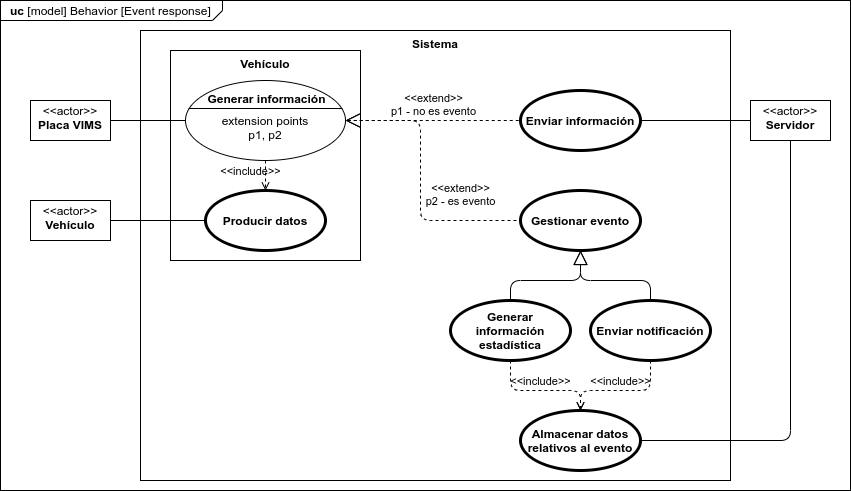
\includegraphics[width=\linewidth]{diagrams/UseCases-UC6 - reaction.png}
  \caption{Caso de uso \texttt{06} -- \textit{generación de eventos}}
  \label{uc:reaction}
\end{figure}

\begin{table}[H]
  \centering
  \begin{tabularx}{\textwidth}{|c|c|X|}
    \hline
    \texttt{06}                                & \multicolumn{2}{c|}{\textit{Generación de eventos}}                                                                                                                                                                                                                                                                         \\
    \hline
    \textbf{Descripción}                       & \multicolumn{2}{X|}{El dispositivo \ac{VIMS}, a la hora de enviar datos, podrá producir eventos según el tipo de información que haya de enviar.}                                                                                                                                                                           \\
    \hline
    \multirow{10}{*}{\textbf{Secuencia normal}} & \textbf{Paso}                                                                                                                                     & \textbf{Acción}                                                                                                                                                         \\
    \cline{2-3}
                                               & 1                                                                                                                                                 & \multicolumn{1}{L|}{El dispositivo \ac{VIMS} genera información y la transmite hacia el servidor.}                                                                      \\
    \cline{2-3}
                                               & 1.1                                                                                                                                               & \multicolumn{1}{L|}{Si la información a transmitir es ``normal'', se envía directamente al servidor.}                                                                   \\
    \cline{2-3}
                                               & 1.2                                                                                                                                               & \multicolumn{1}{L|}{Si la información a transmitir es eventual, se procesa el evento generando información estadística referente al mismo o mandando una notificación.} \\
    \cline{2-3}
                                               & 2                                                                                                                                                 & \multicolumn{1}{L|}{El servidor recibe el evento y se encarga de gestionarlo, como se vio en el \texttt{UC-04}.} \\
    \hline
    \multirow{3}{*}{\textbf{Excepciones}}     & \textbf{Paso}                                                                                                                                     & \textbf{Acción}                                                                                                                                                         \\
    \cline{2-3}
                                               & 1                                                                                                                                               & \multicolumn{1}{L|}{No hay ninguna cuenta asociada al dispositivo.}                                                                                                                    \\
    \cline{2-3}
                                               & 1.1                                                                                                                                               & \multicolumn{1}{L|}{No hay conexión a Internet por parte del dispositivo \ac{VIMS}.}                                                                                    \\
    \hline
  \end{tabularx}
\end{table}

\noindent\rule{\linewidth}{.2pt}

\begin{figure}[H]
  \centering
  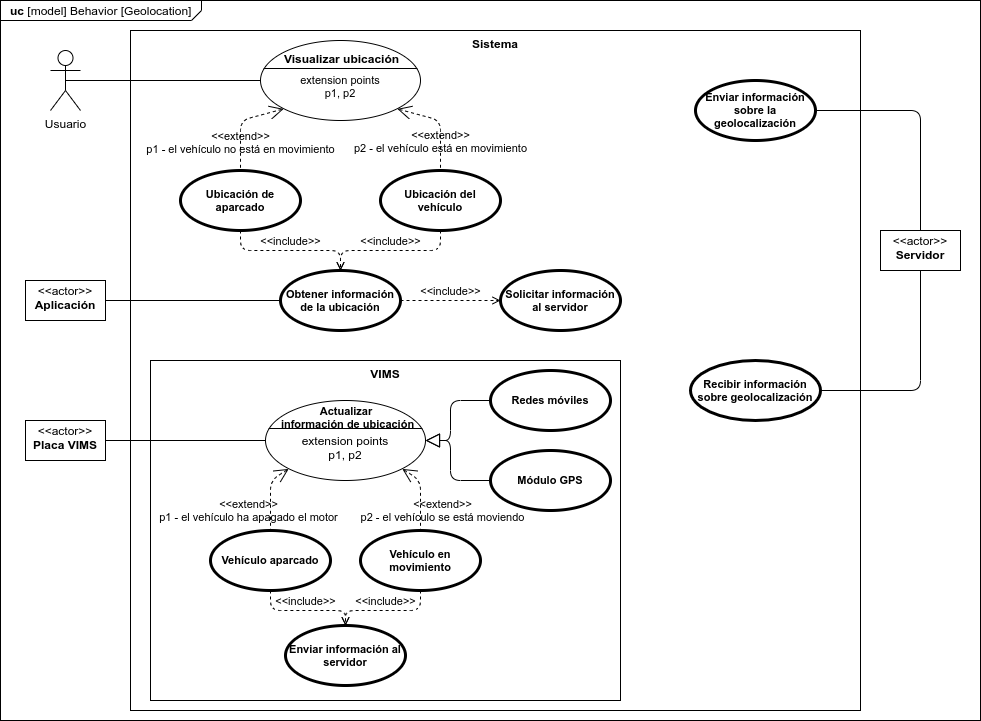
\includegraphics[width=\linewidth]{diagrams/UseCases-UC7 - location.png}
  \caption{Casos de uso \texttt{07*} -- \textit{envío, almacenamiento y visualización de geolocalización}}
  \label{uc:location}
\end{figure}

\begin{table}[H]
  \centering
  \begin{tabularx}{\textwidth}{|c|c|X|}
    \hline
    \texttt{06}                                & \multicolumn{2}{c|}{\textit{Generación de eventos}}                                                                                                                                                                                                                                                                         \\
    \hline
    \textbf{Descripción}                       & \multicolumn{2}{X|}{El dispositivo \ac{VIMS}, a la hora de enviar datos, podrá producir eventos según el tipo de información que haya de enviar.}                                                                                                                                                                           \\
    \hline
    \multirow{10}{*}{\textbf{Secuencia normal}} & \textbf{Paso}                                                                                                                                     & \textbf{Acción}                                                                                                                                                         \\
    \cline{2-3}
                                               & 1                                                                                                                                                 & \multicolumn{1}{L|}{El dispositivo \ac{VIMS} genera información y la transmite hacia el servidor.}                                                                      \\
    \cline{2-3}
                                               & 1.1                                                                                                                                               & \multicolumn{1}{L|}{Si la información a transmitir es ``normal'', se envía directamente al servidor.}                                                                   \\
    \cline{2-3}
                                               & 1.2                                                                                                                                               & \multicolumn{1}{L|}{Si la información a transmitir es eventual, se procesa el evento generando información estadística referente al mismo o mandando una notificación.} \\
    \cline{2-3}
                                               & 2                                                                                                                                                 & \multicolumn{1}{L|}{El servidor recibe el evento y se encarga de gestionarlo, como se vio en el \texttt{UC-04}.} \\
    \hline
    \multirow{3}{*}{\textbf{Excepciones}}     & \textbf{Paso}                                                                                                                                     & \textbf{Acción}                                                                                                                                                         \\
    \cline{2-3}
                                               & 1                                                                                                                                               & \multicolumn{1}{L|}{No hay ninguna cuenta asociada al dispositivo.}                                                                                                                    \\
    \cline{2-3}
                                               & 1.1                                                                                                                                               & \multicolumn{1}{L|}{No hay conexión a Internet por parte del dispositivo \ac{VIMS}.}                                                                                    \\
    \hline
  \end{tabularx}
\end{table}